% Adjust these for the path of the theme and its graphics, relative to this file
%\usepackage{beamerthemeFalmouthGamesAcademy}
\usepackage{../../beamerthemeFalmouthGamesAcademy}
\usepackage{multimedia}
\graphicspath{ {../../} }

% Default language for code listings
\lstset{language=C++,
	morekeywords={each,in,nullptr}
}

\input{../listings_GLSL}

% For strikethrough effect
\usepackage[normalem]{ulem}
\usepackage{wasysym}

\usepackage{pdfpages}

% http://www.texample.net/tikz/examples/state-machine/
\usetikzlibrary{arrows,automata}

\newcommand{\modulecode}{COMP260}\newcommand{\moduletitle}{Distributed Systems}\newcommand{\sessionnumber}{5}

\begin{document}
\title{\sessionnumber: Post-processing}
\subtitle{\modulecode: \moduletitle}

\frame{\titlepage} 

\begin{frame}
	\frametitle{Learning outcomes}
	\begin{itemize}
		\item \textbf{Understand} Post-processing in computer graphics
		\item \textbf{Implement} graphical effects from COMP120 in realtime 
		\item \textbf{Implement} other Post-processing effects in your application
	\end{itemize}
\end{frame}

\part{Introduction}
\frame{\partpage}

\begin{frame}{What is Post-Processing?}
	\begin{itemize}
		\pause\item Is a series of techniques that are carried out after a scene has been rendered
		\pause\item Traditionally this could only be done as an offline process
		\pause\item With the advent of faster GPUs and programmable shaders, we could implement some of the effects in real time
		\pause\item The key to the effect is to switch from drawing to the back buffer to a texture
		\pause\item This texture will contain the scene
		\pause\item We then use a shader to implement a post-processing effect
		\pause\item We then map the processed texture onto a full screen quad, which is rendered to the backbuffer
	\end{itemize}
\end{frame}
\part{Rendering To Texture}
\frame{\partpage}

\begin{frame}{Brief Overview}
	\begin{enumerate}
		\item\pause Create a Texture of the required dimensions
		\item\pause Create Depth Buffer Object
		\item\pause Create a Frambuffer Object (FBO)
		\item\pause Bind the texture and the Depth Buffer Object into the FBO
		\item\pause Bind the FBO to the pipeline
		\item\pause Render the scene to the new framebuffer
	\end{enumerate}
\end{frame}

\begin{frame}[fragile]{Creating a Texture}
	\begin{lstlisting}
//The texture we are going to render to
GLuint renderTextureID;
glGenTextures(1,&renderTextureID);

//Bind Texture
glBindTexture(GL_TEXTURE_2D, renderTexture);

//fill with empty data
glTexImage2D(GL_TEXTURE_2D,0,GL_RGB,
	840,680,0,GL_RGB, GL_UNSIGNED_BYTE,0);

//Add any texture states (filtering etc)
	\end{lstlisting}
\end{frame}

\begin{frame}[fragile]{Creating Depth Buffer Object}
	\begin{lstlisting}
//The depth buffer
GLuint depthBufferID;
glGenRenderbuffers(1,&depthBufferID);

//Bind the depth buffer
glBindRenderbuffer(GL_RENDERBUFFER, depthBufferID);
//Set the foremat of the depth buffer
glRenderbufferStorage(GL_RENDERBUFFER,GL_DEPTH_COMPONENT,
				840,680);
	\end{lstlisting}
\end{frame}

\begin{frame}[fragile]{Creating Frame Buffer}
	\begin{lstlisting}
//The frambuffer
GLuint frameBufferID;
glGenFramebuffers(1,&frameBufferID);
	\end{lstlisting}
\end{frame}

\begin{frame}[fragile]{Bind Texture and Depth Buffer}
	\begin{lstlisting}
//Bind the framebuffer
glBindFramebuffer(GL_FRAMEBUFFER,frameBufferID);

//Bind the texture as a colour attachment 0 to the
//active framebuffer
glFramebufferTexture(GL_FRAMEBUFFER, GL_COLOR_ATTACHMENT0,
				renderTextureID, 0);

//Bind the depth buffer as a depth attachment
glFramebufferRenderbuffer(GL_FRAMEBUFFER,
	GL_DEPTH_ATTACHMENT, GL_RENDERBUFFER, depthBufferID);

if (glCheckFramebufferStatus(GL_FRAMEBUFFER) !=
	GL_FRAMEBUFFER_COMPLETE)
{
	//error message!
}
	\end{lstlisting}
\end{frame}


\begin{frame}[fragile]{Render to Framebuffer}
	\begin{lstlisting}
//Bind the framebuffer
glBindFramebuffer(GL_FRAMEBUFFER, frameBufferID);

//Drawn everything as normal!
	\end{lstlisting}
\end{frame}

\part{Using Our Texture}
\frame{\partpage}

\begin{frame}{Brief Overview}
	\begin{itemize}
		\item\pause Now we have our scene stored on a texture
		\item\pause We need to map this texture onto a surface
		\item\pause This is usually a screen-aligned quad, but it can be any 3D object!
		\item\pause In the fragment shader, we can do some processing...
	\end{itemize}
\end{frame}

\begin{frame}{Steps}
	\begin{enumerate}
		\item\pause Create a Vertex Buffer Object (VBO) for our quad
		\item\pause Create a Vertex Array Object (VAO)
		\item\pause Load in a 'pass through' vertex shader and a fragment shader which takes in a texture
		\item\pause Render the quad and send across the texture that was bound to the framebuffer
	\end{enumerate}
\end{frame}

\begin{frame}[fragile]{Creating our Vertex Buffer Object}
	\begin{lstlisting}
float quadVertices[] =
{
	-1, -1,
	1, -1,
	-1, 1,
	1, 1,
};

GLuint screenQuadVBOID;
glGenBuffers(1, &screenQuadVBOID);
glBindBuffer(GL_ARRAY_BUFFER, screenQuadVBOID);
glBufferData(GL_ARRAY_BUFFER, 8 * sizeof(float), quadVertices,
			GL_STATIC_DRAW);
	\end{lstlisting}
\end{frame}

\begin{frame}[fragile]{Creating our Vertex Array}
	\begin{lstlisting}
GLuint screenVAOID;
glGenVertexArrays(1, &screenVAOID);
glBindVertexArray(screenVAOID);
glBindBuffer(GL_ARRAY_BUFFER, screenQuadVBOID);

glEnableVertexAttribArray(0);
glVertexAttribPointer(0, 2, GL_FLOAT, GL_FALSE, 0, NULL);
	\end{lstlisting}
\end{frame}

\begin{frame}[fragile]{Pass Through Vertex Shader}
	\begin{lstlisting}
#version 330 core

layout(location=0) in vec2 vertexPosition;

out vec2 textureCoords;

void main()
{
	//Calculate Texture Coordinates for the Vertex
	textureCoords = (vertexPosition + 1.0) / 2.0;
	gl_Position = vec4(vertexPosition, 0.0, 1.0);
}
	\end{lstlisting}
\end{frame}

\begin{frame}[fragile]{Example Fragment Shader}
	\begin{lstlisting}
#version 330 core

out vec4 color;
in vec2 textureCoords;

uniform sampler2D texture0;

void main()
{
	//Read the texture and do some processing!
	color = texture(texture0, textureCoords);
}
	\end{lstlisting}
\end{frame}

\begin{frame}[fragile]{Rendering}
	\begin{lstlisting}
glBindFramebuffer(GL_FRAMEBUFFER,0);
glBindVertexArray(screenVAOID);
glBindTexture(GL_TEXTURE_2D, renderTextureID);
// etc.

//Bind our Postprocessing Program

//Send across any values to the shader

//Draw the quad!
	\end{lstlisting}
\end{frame}
\part{COMP120 Refresher}
\frame{\partpage}

\begin{frame}{Image Processing Techniques}
	\begin{itemize}
		\item\pause Some of the algorithms you learned in COMP120 can be applied in GLSL:
		\begin{itemize}
			\item Colour Replacement
			\item Luminance calculation  
			\item Colour Correction
			\item Black \& White and Sepia Tone
			\item Edge Detection
		\end{itemize}
		\pause\item Key difference: we access the data via \textbf{texture coordinates}, rather than array indices.
	\end{itemize}
\end{frame}

\begin{frame}{Modifying Textures}
	\begin{itemize}
		\item\pause A Texture Lookup uses the texture coordinates passed to the fragment shader
		\item\pause Additionally, the fragment shader only processes a single fragment at a time
		\item\pause If we want to access a pixel adjacent to the current one, we can offset the current texture coordinates - this is especially useful for edge detection
		\item\pause GLSL has lots of inbuilt functions (e.g distance) which can aid in creating post-processing effects
	\end{itemize}
\end{frame}
\part{Other Post Processing Techniques}
\frame{\partpage}

  \begin{frame}
	\frametitle{Colour Correction}
	\begin{columns}
		\begin{column}{0.5\textwidth}
			\begin{itemize}
				\item Process of taking an image, convert each colour in the image to a some other colour
				\item Mimic a specific film stock, provide coherent look or provide a mood
			\end{itemize}
		\end{column}
		\begin{column}{0.5\textwidth}
			\begin{center}
				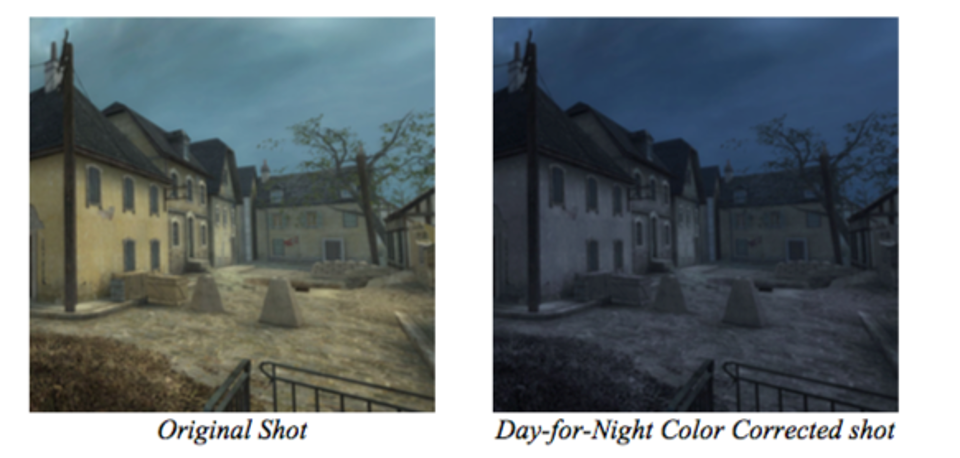
\includegraphics[width=\textwidth]{colour_correction_daynight}
			\end{center}
		\end{column}
	\end{columns}
\end{frame}


\begin{frame}
	\frametitle{Colour Correction Again}
		\begin{columns}
		\begin{column}{0.5\textwidth}
			\begin{itemize}
				\item Depending on the technique this could involve manipulating the colours using a Filter Kernel
				\item Or we could use a colour palette (see Colour Grading) 
			\end{itemize}
		\end{column}
		\begin{column}{0.5\textwidth} 
			\begin{center}
				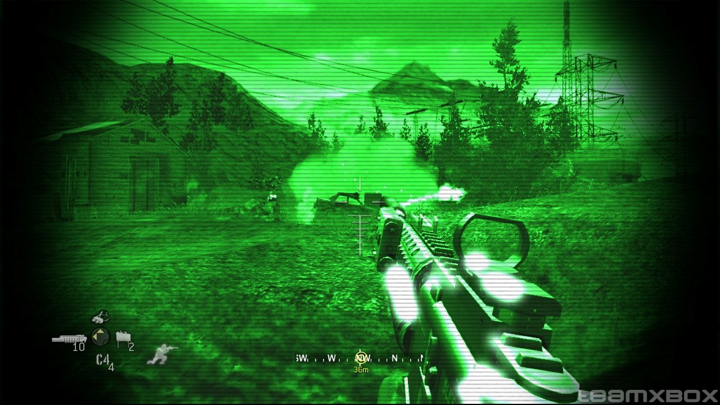
\includegraphics[width=\textwidth]{colour_correction_nightvision}
			\end{center}
		\end{column}
	\end{columns}
\end{frame}

\begin{frame}{Blur}
	\begin{itemize}
		\item\pause This often used as a basis for other techniques such as Depth of Field and HDR
		\item\pause To achieve blurring we apply a filter to the texture lookup of the texture render target
		\item\pause We can apply many different filters, one of the simplest is a Box Filter
		\item\pause With a box filter we sample 4 points around the point we are interested in
	\end{itemize}
\end{frame}

\begin{frame}
	\frametitle{Motion Blur}
\begin{columns}
	\begin{column}{0.5\textwidth}
		\begin{itemize}
			\item If an object moves very fast through you Field of view it can appear that the object leaves a slight ghost of itself
			\item There are several ways of implementing this, we can use the actual speed of the object to determine the amount of blur
		\end{itemize}
	\end{column}
	\begin{column}{0.5\textwidth} 
		\begin{center}
			
\includegraphics[width=\textwidth]{motion_blur}
		\end{center}
	\end{column}
\end{columns}
\end{frame}

\begin{frame}
	\frametitle{Motion Blur}
	\begin{columns}
		\begin{column}{0.5\textwidth}
			\begin{itemize}
				\item Or we can simply take the results of the last render update and blend them with current render results and blend based on a lerp
			\end{itemize}
		\end{column}
		\begin{column}{0.5\textwidth} 
			\begin{center}
				
\includegraphics[width=\textwidth]{motion_blur}
			\end{center}
		\end{column}
	\end{columns}
\end{frame}

\begin{frame}
	\frametitle{Depth of Field}
\begin{columns}
	\begin{column}{0.5\textwidth}
		\begin{itemize}
			\item DOF attempts to simulate the effect where object that are too close or too far away appear out of focus
			\item We first have to consider in our scene what range of depth values will be considered in focus. We then need to blur everything that is outside this range
		\end{itemize}
	\end{column}
	\begin{column}{0.5\textwidth} 
		\begin{center}
			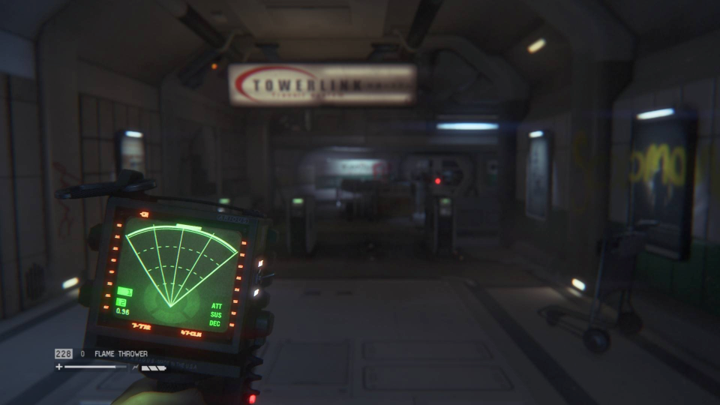
\includegraphics[width=\textwidth]{depth_of_field}
		\end{center}
	\end{column}
\end{columns}	
\end{frame}

\begin{frame}
	\frametitle{Depth of Field}
	\begin{columns}
		\begin{column}{0.5\textwidth}
			\begin{itemize}
				\item Once we have determined this we render a blurred scene to a render texture
			\end{itemize}
		\end{column}
		\begin{column}{0.5\textwidth} 
			\begin{center}
				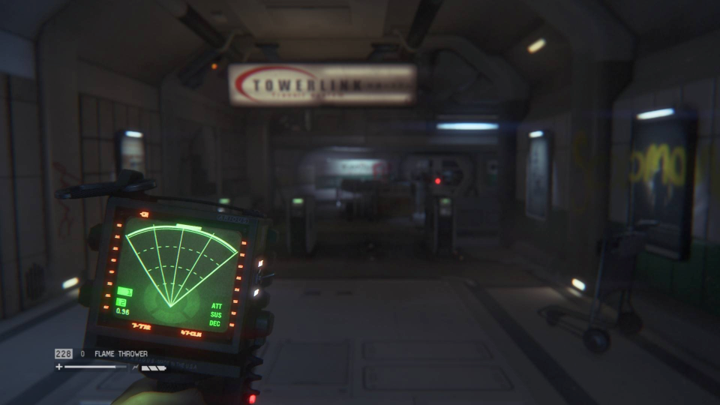
\includegraphics[width=\textwidth]{depth_of_field}
			\end{center}
		\end{column}
	\end{columns}	
\end{frame}

\begin{frame}
	\frametitle{Bloom}
	\begin{columns}
		\begin{column}{0.5\textwidth}
			\begin{itemize}
				\item This attempts to simulate the overloading of the optic nerve if extremely bright areas of a surface are visible
				\item First of we render to a smaller render target usually 1/4 size
			\end{itemize}
		\end{column}
		\begin{column}{0.5\textwidth} 
			\begin{center}
				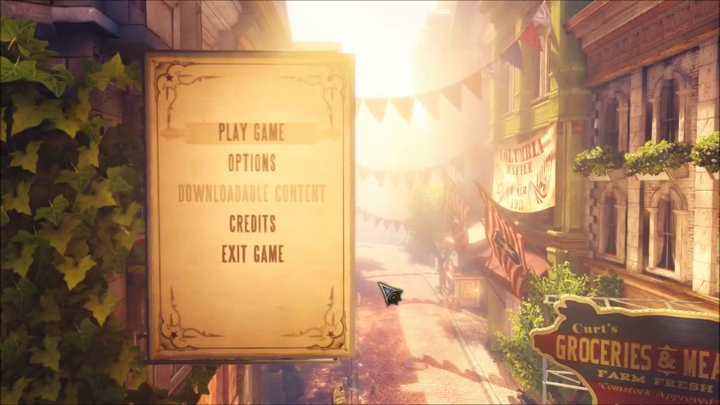
\includegraphics[width=\textwidth]{bloom}
			\end{center}
		\end{column}
	\end{columns}	
\end{frame}

\begin{frame}
	\frametitle{Bloom}
	\begin{columns}
		\begin{column}{0.5\textwidth}
			\begin{itemize}
				\item We then apply a filter(usually Gauss) to this reduced render target, if we apply this filter of multiple passes then we achieve a smoother blur
				\item We then blend the blurred image onto the screen with the original scene 
			\end{itemize}
		\end{column}
		\begin{column}{0.5\textwidth} 
			\begin{center}
				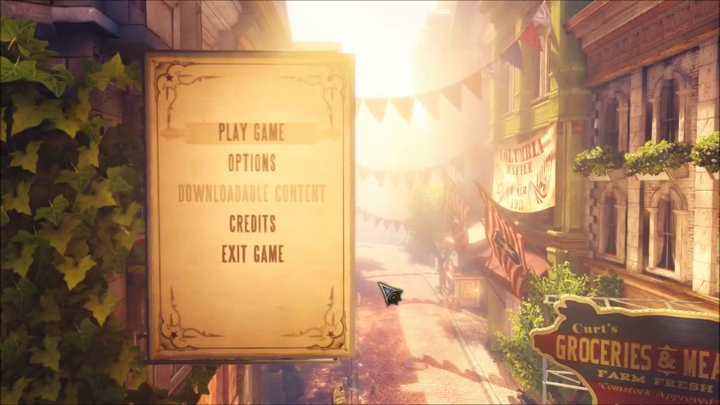
\includegraphics[width=\textwidth]{bloom}
			\end{center}
		\end{column}
	\end{columns}	
\end{frame}
\input{debrief}
\part{Exercises}
\frame{\partpage}

\begin{frame}{Exercise 1 - Texturing}
	\begin{itemize}
		\item Load in a image using SDL Image
		\item Copy this image into a OpenGL Texture
		\item Add Texture Coordinates to your Cube or Square
		\item Map this texture onto the Cube or Square
		\item Finally change the texture to a transparent texture
	\end{itemize}
\end{frame}

\begin{frame}{Exercise 2 - Model Loading}
	\begin{itemize}
		\item Create the following NFF models and load each one to the screen
		\begin{itemize}
			\item Tetrahedron 
			\item Cube
			\item Sphere
			\item Cylinder
		\end{itemize}
		\item \url{http://assimp.sourceforge.net/howtoBasicShapes.html}
		\item \url{https://github.com/assimp/assimp/tree/master/test/models/NFF/NFF}
	\end{itemize}
\end{frame}

\begin{frame}{Exercise 3 - More Complex Scene}
	\begin{itemize}
		\item Create a GameObject class which contains the following as member variables
		\begin{itemize}
			\item Vertex Buffer
			\item Element Buffer
			\item Vertex Array Object
			\item Position, Scale, Rotation Vectors
			\item Position, Scale, Rotation, Model Matrices
			\item Open GL Texture
			\item Number of vertices and Indices
		\end{itemize}
		\item Add in functions to initialise and get each of these values
		\item Add in functions to update (calculate the model matrix) and render
		\item Create an instance of this Game Object and display it on the screen
	\end{itemize}
\end{frame}

\end{document}
